\subsection{UC16 - Rimozione di un alert}
\begin{figure}[H]
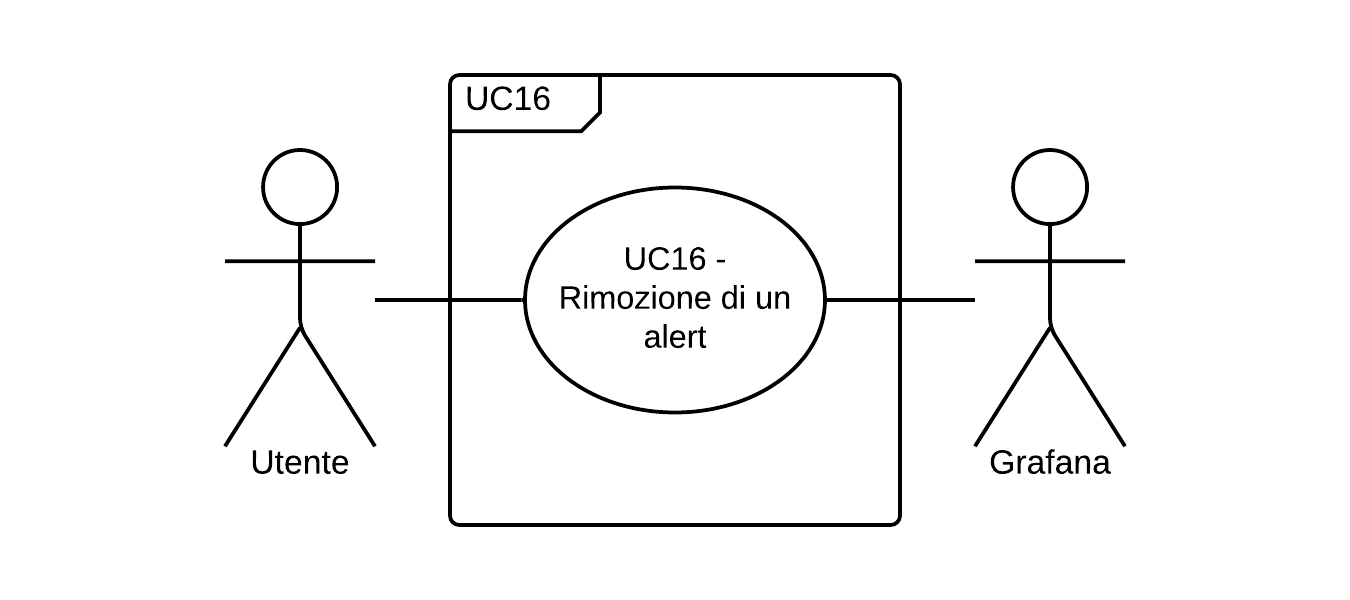
\includegraphics{img/UC16_-_Rimozione_di_un_alert.png}
\caption{Diagramma degli use case di UC16}
\end{figure}
\begin{itemize}
	\item \textbf{Codice identificativo}: UC16;
	\item \textbf{Titolo}: rimozione di un alert\glo;
	\item \textbf{Attore primario}: utente;
	\item \textbf{Attore secondario}: Grafana\glo;
	\item \textbf{Descrizione}: l'utente rimuove un alert\glosp da un pannello grafico;
	\item \textbf{Precondizione}: l'utente è autenticato nel sistema software Grafana\glosp ed ha inserito e selezionato almeno un alert\glo;
	\item \textbf{Postcondizione}: l'alert\glosp selezionato dall'utente è eliminato;
	\item \textbf{Scenario principale}: utilizzando l'apposita funzione offerta da Grafana\glo, l'utente elimina l'alert\glosp che ha selezionato.
\end{itemize} 
